\subsection{Result analyzing - Draft}

Correlation coefficients are used in statistics to measure how strong a relationship is between two variable space. Concretely, in this case those variable space are Semantic score and RUBY. 


We aim to figure out specifics of a dataset in which RUBY can work well. Because RUBY was created to estimate the semantic of code translation, the dataset in which RUBY works well also is the dataset containing the high correlation between Semantic score and RUBY. 

\subsubsection{Using RANSAC}
The RANSAC (Random Sample Consensus) algorithm~\cite{ Fischler:1981:RSC:358669.358692} is a simple, yet powerful, technique that is commonly applied to the task of estimating the parameters of a model, using data that may be contaminated by outliers. RANSAC estimates a global relation that fits the data, while simultaneously classifying the data into inliers (points consistent with the relation) and outliers (points not consistent with the relation). Due to its ability to tolerate a large fraction of outliers, the algorithm is a popular choice for a variety of robust estimation problems.


RANSAC assumes that the training data consists of inliers that can be explained with the model and outliers that are gross-erroneous samples which don't fit the model at all. So using outliers when training the model would increase our final prediction error, as they contain almost no information about the model. Therefore, in our research scope, we use RANSAC as a mean of classification data which includes points contributing to the correlation of the method (inliers) and points decreasing the correlation of the method (outliers).

\subsubsection{Experiments}
We conducted 10 experiments with RANCSAC running on the same dataset from our result.  (Table~\ref{table:RANSAC_experiments}) shows results of our 10 experiments which contains the number of inlier points and the correlations of those inliers. According to the outcome, we chose the dataset result with the median of correlation that is No5 in the table for analyzing and finding out the specifics of that dataset. Figure~\ref{fig:inliers_outliers} shows the result of experiment No5.
\begin{table}
	\caption{RANSAC experiments}
	\begin{tabular}{|c|c|c|c|c|}
		\hline
		Experiment Number & Number of inliers & Correlations of inliers \\
		\hline
		10	& 315	& 0.934700727 \\		
		8	& 312	& 0.945424846 \\	
		9	& 312	& 0.947983773 \\
		4	& 310	& 0.948196013 \\
		{\cellcolor[gray]{.8}}5	& {\cellcolor[gray]{.8}}308	& {\cellcolor[gray]{.8}}0.954874293 \\
		7	& 244	& 0.955112418 \\	
		1	& 283	& 0.957661146 \\
		3	& 303	& 0.958122675 \\
		2	& 298	& 0.958659967 \\
		6	& 277	& 0.959811603 \\		
		\hline
	\end{tabular}
	\label{table:RANSAC_experiments}
\end{table}

\begin{figure}[t]
	\caption{An example: Dataset in experiment No5 classified into inlier points(green) and outlier point(yellow)}
	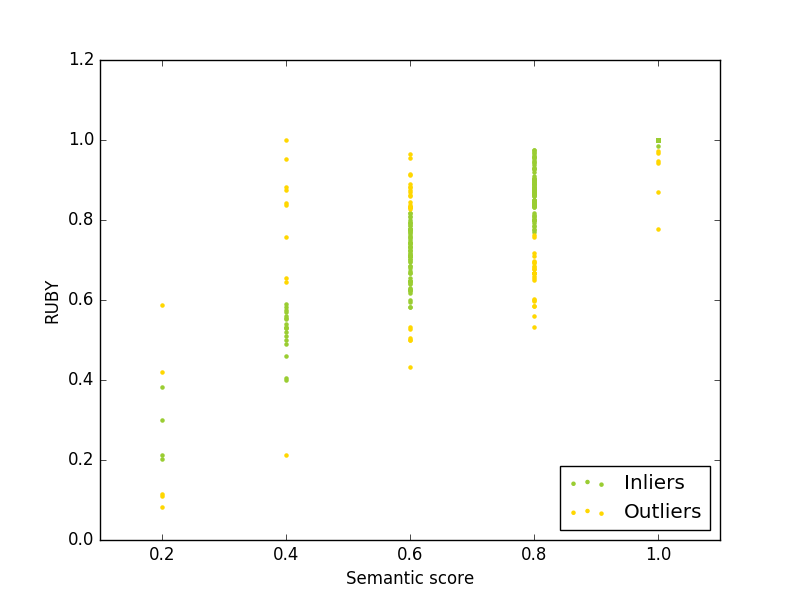
\includegraphics[scale=0.4]{img/inliers_outliers.png}
	\centering
	\label{fig:inliers_outliers}
\end{figure}

\subsubsection{Result classification}
We manually classify the method set of the inlier points into serveral categories based on the relation between the method and its reference. Table~\ref{table:result_classification} shows the result of classification for our set of data.
\begin{table}
	\caption{Result classification}
	  \scalebox{1}{
		\begin{tabular}{|c|m{4.5cm}|}
			\hline
			Method category & Description \\
			\hline
			IDENTIDFIED\_CODE	& Code is the same with the reference \\		
			\hline
			SAME\_FUNC\_DIFF\_LEX	& FQN vs PN, For vs Foreach, [i] vs .get(i) \\		
			\hline
			SAME\_DATA\_FLOW	& Same data flow but there are still incorrect piece of code \\	
			\hline
			DISORDERED\_CODE & Several same pieces of code was disordered \\		
			\hline
			SAME\_API\_NAME & Code includes the same APIs and params name with its reference but incorrect usages \\
			\hline
			SAME\_SOME\_LOC & There are some lines of code which are same with the reference \\
			\hline
			DIFFERENT\_CODE & Code is totally different from the its reference \\
			\hline
		\end{tabular}
	}
		\label{table:result_classification}
\end{table}